% gc-07-HigherOrder.tex

\documentclass[xcolor=dvipsnames]{beamer}
\usepackage{teachbeamer}

\title{Higher-Order Derivatives}
\subtitle{{\CourseNumber}, BCIT}

\author{\CourseName}

\date{January 29, 2018}

% \begin{figure}[h]
% 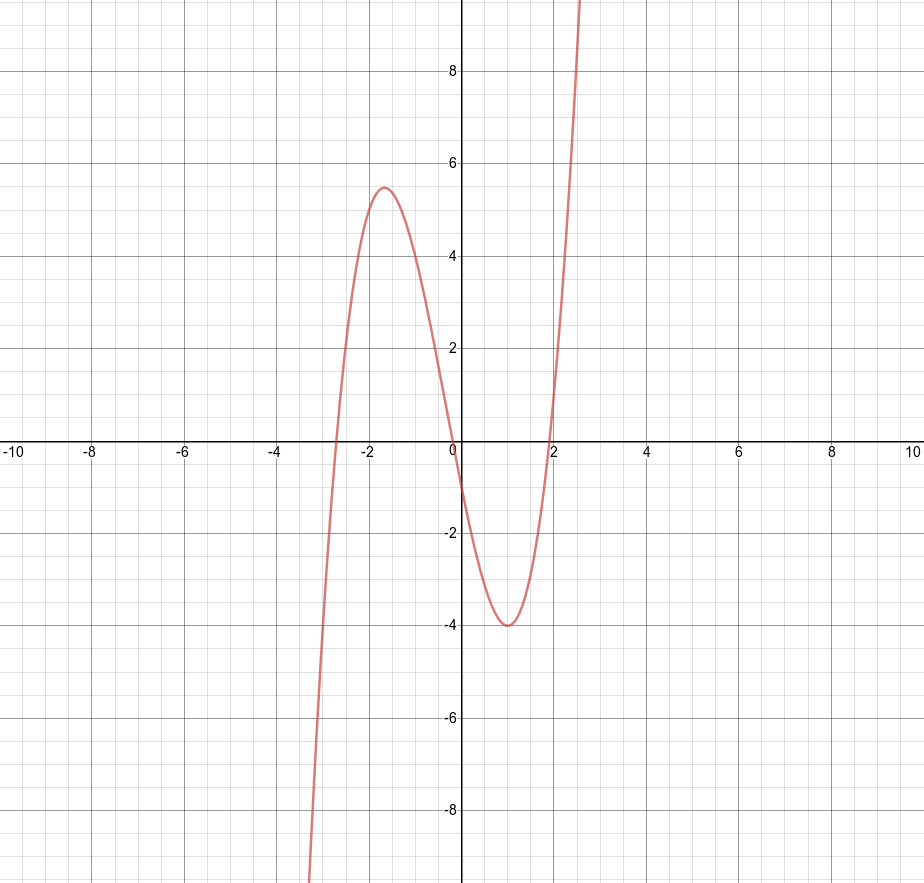
\includegraphics[scale=.3]{./diagrams/extrema1.png}
% \end{figure}

\begin{document}

\begin{frame}
  \titlepage
\end{frame}

\begin{frame}
  \frametitle{Expanding the Logarithm}
The logarithm is only defined on the positive real numbers. It turns
out that
\begin{equation}
  \label{eq:feegeigu}
  \frac{d}{dx}\ln\vert{}x\vert=\frac{1}{x}\mbox{ for all real numbers except }x=0
\end{equation}
Remember that the absolute value $\vert{}x\vert$ is defined as
\begin{equation}
  \label{eq:iegeecie}
  \vert{}x\vert=\left\{
    \begin{array}{l}
      x\mbox{ for }x\geq{}0 \\
      -x\mbox{ for }x<0
    \end{array}\right.
\end{equation}
\end{frame}

\begin{frame}
  \frametitle{Differentiating the Absolute Value}
Treat functions with an absolute value as you would treat piecewise
defined functions. A piecewise defined function looks like this:
\begin{equation}
  \label{eq:iboashaz}
  f(x)=\left\{
    \begin{array}{l}
      x^{2}-7\mbox{ for }x>7 \\
      e^{1/x}\mbox{ for }x\leq{}7
    \end{array}\right.
\end{equation}
Now differentiate
\begin{equation}
  \label{eq:aeghooki}
  g(t)=\vert{}t^{2}+t\vert
\end{equation}
\end{frame}

\begin{frame}
  \frametitle{Absolute Value Example}
Differentiate
\begin{equation}
  \label{eq:eimufosh}
  f(x)=\vert{}x-1\vert
\end{equation}
You can do this two ways: (a) use the chain rule and
\begin{equation}
  \label{eq:agabooto}
f(x)=\sqrt{(x-1)^{2}}
\end{equation}
(b) use the piecewise definition
\begin{equation}
  \label{eq:ephohnge}
f(x)=\left\{
  \begin{array}{l}
    x-1\mbox{ for }x\geq{}1 \\
    1-x\mbox{ for }x<1
  \end{array}\right.
\end{equation}
\end{frame}

\begin{frame}
  \frametitle{Absolute Value Exercises}
Differentiate
\begin{equation}
  \label{eq:ikaishup}
  f(x)=-x+2+\vert{}-x+2\vert
\end{equation}
\begin{equation}
  \label{eq:emaiyito}
  f(x)=\vert{}2x-5\vert
\end{equation}
\begin{equation}
  \label{eq:deiquohr}
  f(x)=(x-2)^{2}+\vert{}x-2\vert
\end{equation}
\begin{equation}
  \label{eq:leihuwee}
  f(x)=-3\cdot\vert{}x+2\vert{}-1
\end{equation}
\end{frame}

\begin{frame}
  \frametitle{Proving the Power Rule}
We have shown the power rule to be true for $n=2$ and $n=0.5$. Here is
a proof that it is true for all real numbers $n$. Let
\begin{equation}
  \label{eq:taesaeph}
  f(x)=\ln\vert{}x^{n}\vert
\end{equation}
On the one hand,
\begin{equation}
  \label{eq:uzahheir}
  f'(x)=\frac{1}{x^{n}}\frac{d}{dx}x^{n}
\end{equation}
On the other hand, using $f(x)=n\cdot\ln\vert{}x\vert$,
\begin{equation}
  \label{eq:veikoowa}
f'(x)=\frac{n}{x}  
\end{equation}
Consequently,
\begin{equation}
  \label{eq:aebiedah}
  \frac{d}{dx}x^{n}=nx^{n-1}
\end{equation}
\end{frame}

\begin{frame}
  \frametitle{Logarithmic Differentiation}
Using this method, we can differentiate a function such as
\begin{equation}
  \label{eq:ooteiquo}
  f(x)=x^{\sqrt{x}}\mbox{, using the helper function }g(y)=\ln{}x^{\sqrt{x}}
\end{equation}
% Use as a helper function
% \begin{equation}
%   \label{eq:boucheih}
%   g(y)=\ln{}x^{\sqrt{x}}
% \end{equation}
Now use the chain rule for
\begin{equation}
  \label{eq:quuquish}
  g'(y)=\frac{1}{x^{\sqrt{x}}}\frac{d}{dx}x^{\sqrt{x}}
\end{equation}
and the properties of logarithms for
\begin{equation}
  \label{eq:ahfahngi}
  g'(y)=\frac{d}{dx}\left(\sqrt{x}\cdot\ln{}x\right)
\end{equation}
Compare the results and isolate $d/dx(x^{\sqrt{x}})$. Alternatively,
use
\begin{equation}
  \label{eq:gaibahto}
  x^{\sqrt{x}}=\left(e^{\ln{}x}\right)^{\sqrt{x}}
\end{equation}
\end{frame}

\begin{frame}
  \frametitle{Higher-Order Derivatives}
Derivatives often have derivatives themselves, and so on. If $f$ is a
function of time determining the position of an object, then $f'$ is
sometimes called the velocity of the object as a function of time,
$f''$ is called the acceleration of the object as a function of time,
and $f'''$ is called the jerk of the object as a function of time. For
higher-order derivatives than that, we write $f^{(n)}$, for example
\begin{equation}
  \label{eq:zeitohke}
  f(x)=x^{4}+3x^{3}+7x^{2}-\pi{}x+1\mbox{ and }f^{(4)}=24
\end{equation}
\end{frame}

\begin{frame}
  \frametitle{Exercises}
(1) If $g(\vartheta)=\vartheta\sin\vartheta$, find $g''(\pi/6)$.

\bigskip

(2) find $f^{(n)}(x)$ if $f(x)=1/(2-x)$.
\end{frame}

\begin{frame}
  \frametitle{End of Lesson}
Next Lesson: Applications
\end{frame}

\end{document}
